\documentclass[titlepage]{scrartcl}
\usepackage{enumitem}
\usepackage[british]{babel}
\usepackage[style=apa, backend=biber]{biblatex}
\DeclareLanguageMapping{british}{british-apa}
\usepackage{url}
\usepackage{float}
\usepackage{caption}
\restylefloat{table}
\usepackage{perpage}
\MakePerPage{footnote}
\usepackage{abstract}
\usepackage{graphicx}
% Create hyperlinks in bibliography
\usepackage{hyperref}
\usepackage{amsmath}

\usepackage[T1]{fontenc}
\usepackage[utf8]{inputenc}
\usepackage{blindtext}
\setkomafont{disposition}{\normalfont\bfseries}

\graphicspath{
    {./resources/},
}
\addbibresource{~/Documents/library.bib}


\newsavebox{\abstractbox}
\renewenvironment{abstract}
  {\begin{lrbox}{0}\begin{minipage}{\textwidth}
   \begin{center}\normalfont\sectfont\abstractname\end{center}\quotation}
  {\endquotation\end{minipage}\end{lrbox}%
   \global\setbox\abstractbox=\box0 }

\usepackage{etoolbox}
\makeatletter
\expandafter\patchcmd\csname\string\maketitle\endcsname
  {\vskip\z@\@plus3fill}
  {\vskip\z@\@plus2fill\box\abstractbox\vskip\z@\@plus1fill}
  {}{}
\makeatother

\DeclareCiteCommand{\citeyearpar}
    {}
    {\mkbibparens{\bibhyperref{\printdate}}}
    {\multicitedelim}
    {}

% MATLAB Code block stuff...
\usepackage{color}
\usepackage{listings}

\definecolor{dkgreen}{rgb}{0,0.6,0}
\definecolor{gray}{rgb}{0.5,0.5,0.5}

\newcommand{\code}[1]{\texttt{#1}}

\lstset{language=Matlab,
    keywords={break,case,catch,continue,else,elseif,end,for,function,
        global,if,otherwise,persistent,return,switch,try,while},
    basicstyle=\ttfamily,
    keywordstyle=\color{blue},
    commentstyle=\color{gray},
    stringstyle=\color{dkgreen},
    numbers=left,
    numberstyle=\tiny\color{gray},
    stepnumber=1,
    numbersep=10pt,
    backgroundcolor=\color{white},
    tabsize=4,
    showspaces=false,
    showstringspaces=false
    frame=single,
    breaklines=true,
    %postbreak=\raisebox{0ex}[0ex][0ex]{\ensuremath{\color{red}\hookrightarrow\space}}
}

\begin{document}
\title{ECS708P/U - Machine Learning}
\subtitle{\LARGE{Assignment 1 Report\\Linear and Logistic Regression}}
\author{Sam Perry - EC16039}

\maketitle

\section{Linear Regression}
\subsection{Modify the function \code{calculate\_hypothesis.m} to return the predicted value for a single specified training example}
\begin{lstlisting}
function hypothesis = calculate_hypothesis(X, theta, training_example)
    % Calculates the hypothesis for a given X, theta and specified training example
    % Get bias term
    x0 = X(training_example, 1);
    % Get first term
    x1 = X(training_example, 2);

    % Calculate output hypothesis
    hypothesis = theta(1)*x0+theta(2)*x1;
end
\end{lstlisting}\leavevmode \\

\subsection{Notice that the hypothesis function is not being used in the
\code{gradient\_descent} function. Modify this to use the
\code{calculate\_hypothesis} function}
\begin{lstlisting}[firstnumber=27]
        ...
        for i = 1:m
            hypothesis = calculate_hypothesis(X, theta, i);
            output = y(i);
            sigma = sigma + (hypothesis - output);
        end

        theta_0 = theta_0 - ((alpha * 1.0) / m) * sigma;

        sigma = 0.0;

        for i = 1:m
            hypothesis = calculate_hypothesis(X, theta, i);
            output = y(i);
            sigma = sigma + (hypothesis - output) * X(i, 2);
        end
        ...
\end{lstlisting}\leavevmode \\
 
\subsection{Observe what happens when you use a very high or very low learning
rate}
When a very low alpha value ($\alpha=0.0001$) is used, the reduction in cost
per iteration is not sufficient to generate an accurate function. Many more
iterations would be needed to produce a value of $\theta$ close to the desired
local minima. This is illustrated in figures~\ref{LowLearnFunc} and
~\ref{LowLearnCost}.\\

A high value for alpha ($\alpha=1.0$) will result in large shifts in the
function over each iteration. This causes $\theta$ to diverge in the gradient
descent algorithm, increasing between positive and negative values further away
from the minima on each iteration. The final result of this can be seen in
figure~\ref{HighLearnFunc}. The exponential increase in cost causes only the
final increase to be clear through figure~\ref{HighLearnCost}.

\begin{figure}
    \caption{Hypothesis Function ($\alpha=0.0001$)}
    \makebox[\textwidth]{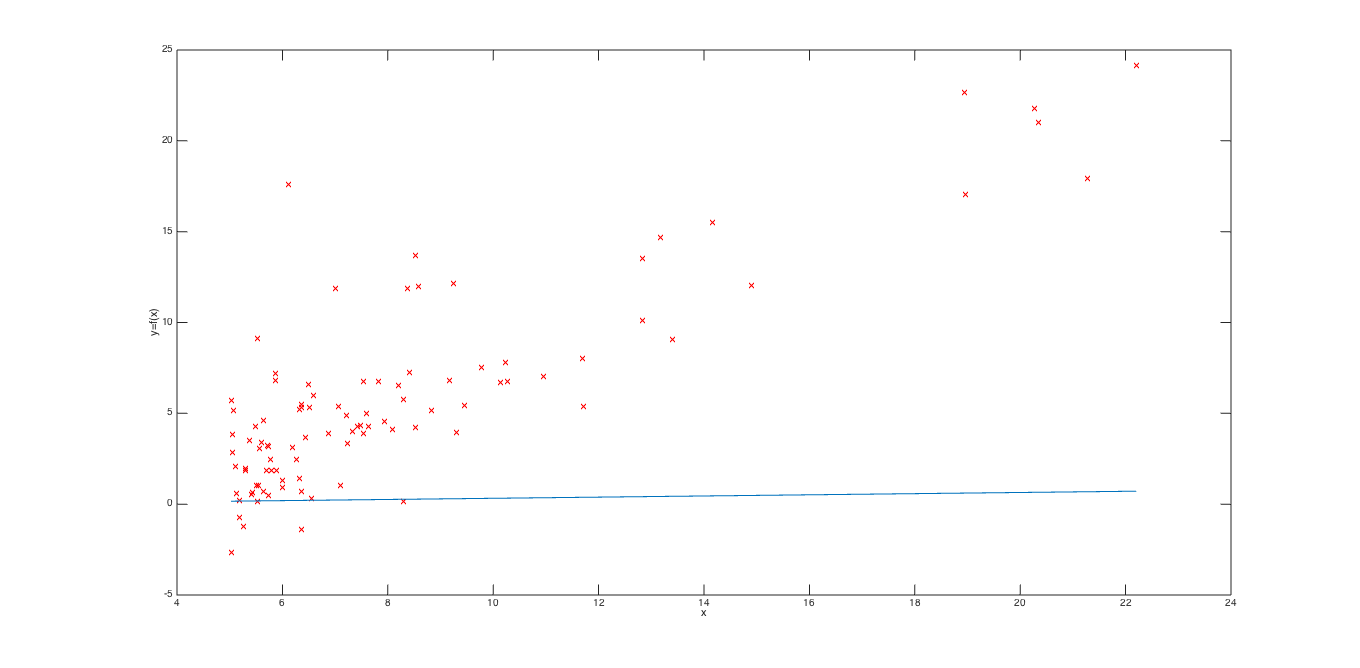
\includegraphics[width=1\textwidth]{LowLearningRateFunc}}
    \label{LowLearnFunc}
    \caption{Cost Function ($\alpha=0.0001$)}
    \makebox[\textwidth]{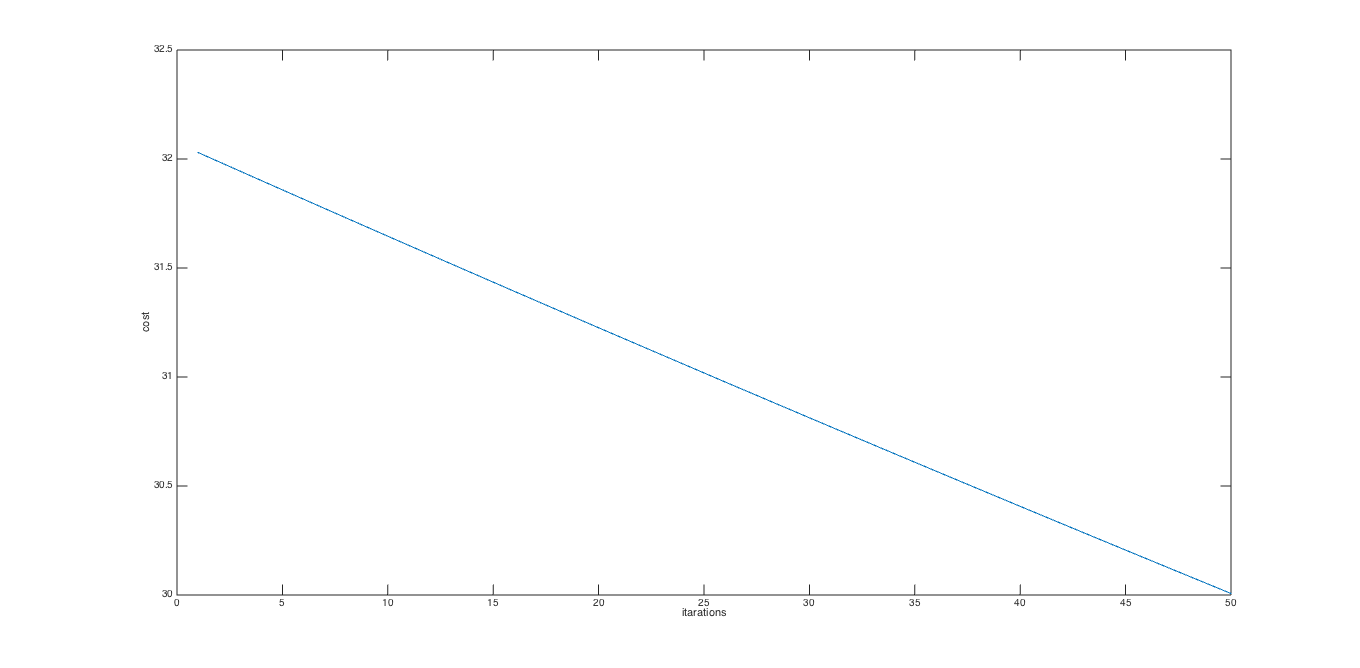
\includegraphics[width=1\textwidth]{LowLearningRateCost}}
    \label{LowLearnCost}
\end{figure}

\begin{figure}
    \caption{Hypothesis Function ($\alpha=1.0$)}
    \makebox[\textwidth]{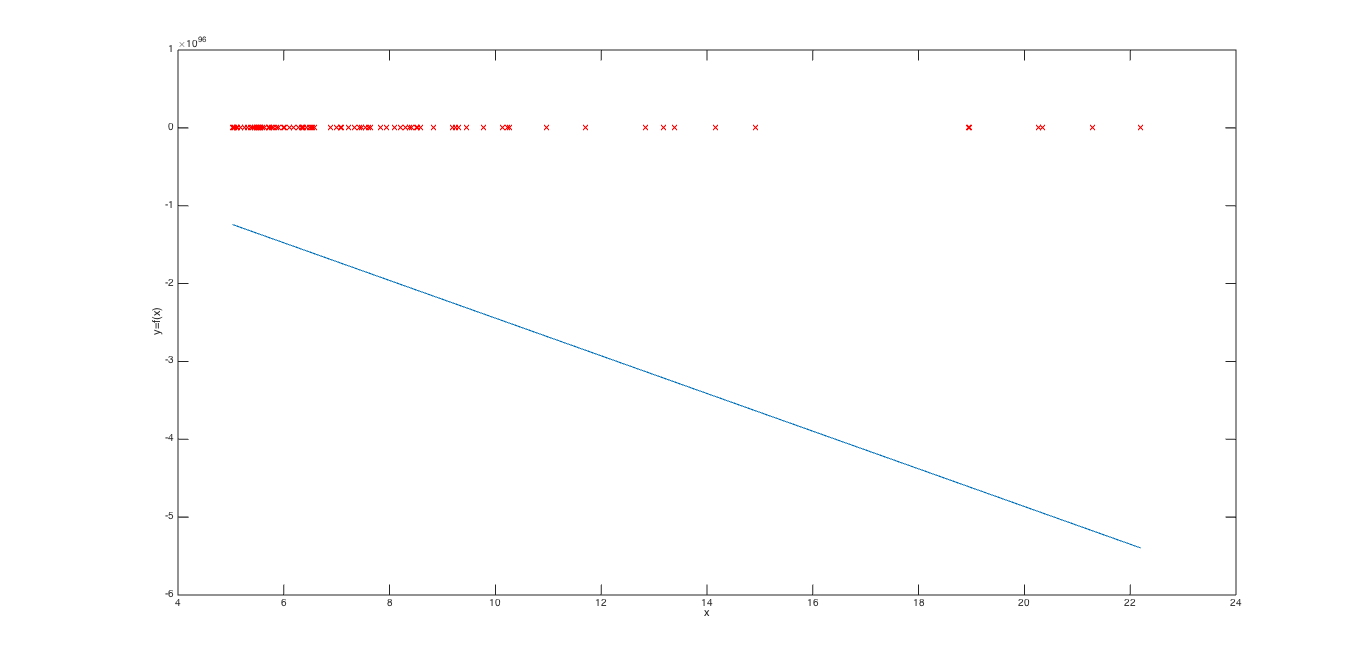
\includegraphics[width=1\textwidth]{HighLearningRateFunc}}
    \label{HighLearnFunc}
    \caption{Cost Function ($\alpha=1.0$)}
    \makebox[\textwidth]{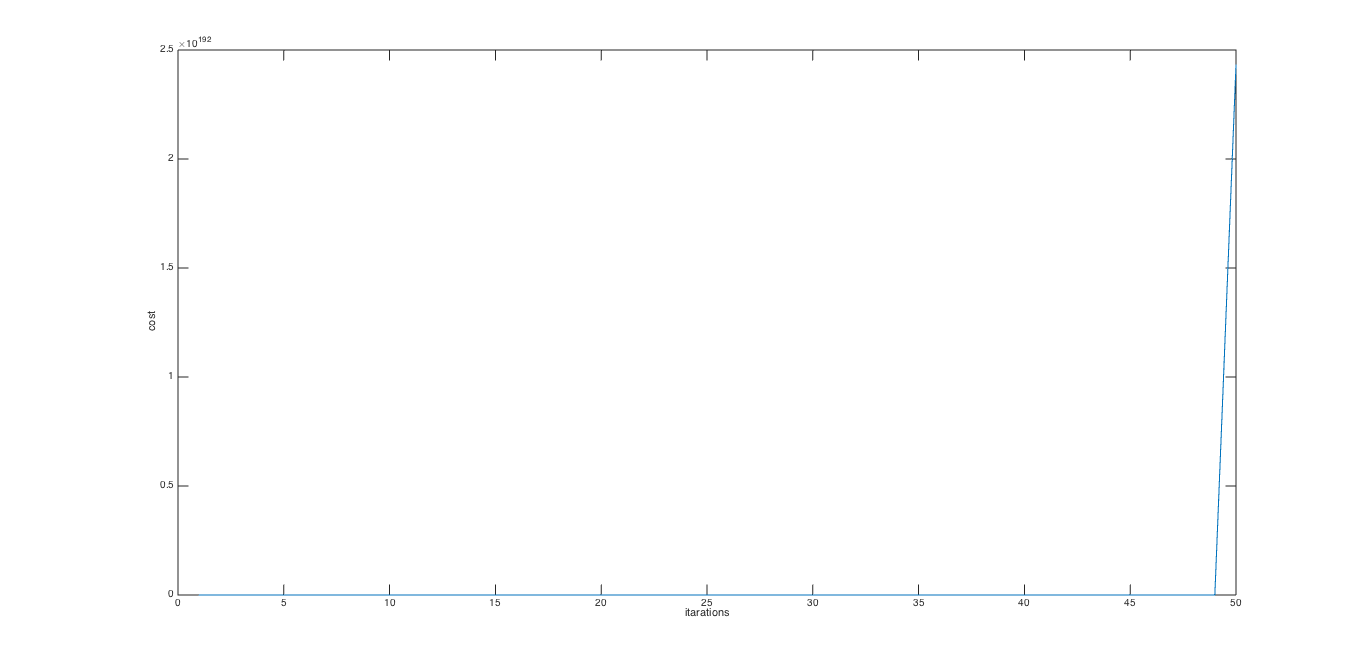
\includegraphics[width=1\textwidth]{HighLearningRateCost}}
    \label{HighLearnCost}
\end{figure}

\subsection{Modify the functions \code{calculate\_hypothesis} and
    \code{gradient\_descent} to support the new hypothesis. This should be
    sufficiently general so that we can have any number of extra variables.}
\begin{lstlisting}
function hypothesis = calculate_hypothesis(X, theta, training_example)
    % CALCULATE_HYPOTHESIS This calculates the hypothesis for a given X,
    % theta and specified training example
    x = X(training_example, 1:length(theta));

    % Calculate the hypothesis as the sum of x values multiplied by there
    % relevant theta values.
    hypothesis = sum(x.*theta);
end
\end{lstlisting}\leavevmode \\

\begin{samepage}
\subsection{Print the theta values found at the end of the optimization. Does anything surprise you?}
The final values for $\theta$ were:\\
$\theta = \big[ 340412.659574468, 110631.050278846, -6649.4742708198 \big]$\\
          
The resulting values of $\theta$ were significantly larger (as was the overall
cost) when using an extra feature than those for computing with only one
feature:\\
$\theta = \big[ -0.263203788443744, 0.82810187360801 \big]$
\end{samepage}

\subsection{How much does you algorithm predict that a house with 1650 sq. ft.
and 3 bedrooms cost? How about 3000 sq. ft. and 4 bedrooms?}

The formula:
$$h_\theta(x)=\theta_0x_0+\theta_1x_1+\theta_2x_2$$

was applied to the new values (pre-normalized) $x_1=1650, x_2=3$ using the calculated
values for $\theta$. From this, a predicted house price of \$293,083 was generated
(rounded to the nearest \$).\\
For values $x_1=3000, x_2=4$ a price of \$472,277 was predicted.

\subsection{modify \code{gradient\_descent} to use the
\code{compute\_cost\_regularised} method instead of \code{computer\_cost}}

\begin{lstlisting}
function theta = gradient_descent(X, y, theta, alpha, iterations, l, do_plot)
...
\end{lstlisting}

\begin{lstlisting}[firstnumber=40]
...
%update cost_vector
cost_vector = [cost_vector; compute_cost_regularised(X, y, theta, l)];
...
\end{lstlisting}\leavevmode \\

\subsection{Modify \code{gradient\_descent} to incorporate the new cost function}

\begin{lstlisting}[firstnumber=23]
...
for ind = 1:length(theta_temp)
    %update theta(1) and store in temporary variable theta_0
    sigma = 0.0;

    for i = 1:m
        hypothesis = calculate_hypothesis(X, theta, i);
        output = y(i);
        sigma = sigma + (hypothesis - output) * X(i, ind);
    end

    % Apply regularization to all terms aside from the bias term.
    if ind > 1
        theta_temp(ind) = (theta_temp(ind) * (1.0-alpha*(l/m))) - ((alpha * 1.0) / m) * sigma;
    else
        theta_temp(ind) = theta_temp(ind) - ((alpha * 1.0) / m) * sigma;
    end
end
...
\end{lstlisting}\leavevmode \\


\subsection{Find the best values of $\alpha$ to use in order to optimize best}
Through trial and error, the value for alpha that best fit the data was found
to be around 1.461. Higher values than this were found to diverge. The cost and
hypothesis functions are shown in figures~\ref{PolynomialAlphaOnlyFunc}
and~\ref{PolynomialAlphaOnlyCost}.

\begin{figure}
    \caption{Hypothesis Function ($\alpha=1.461$)}
    \makebox[\textwidth]{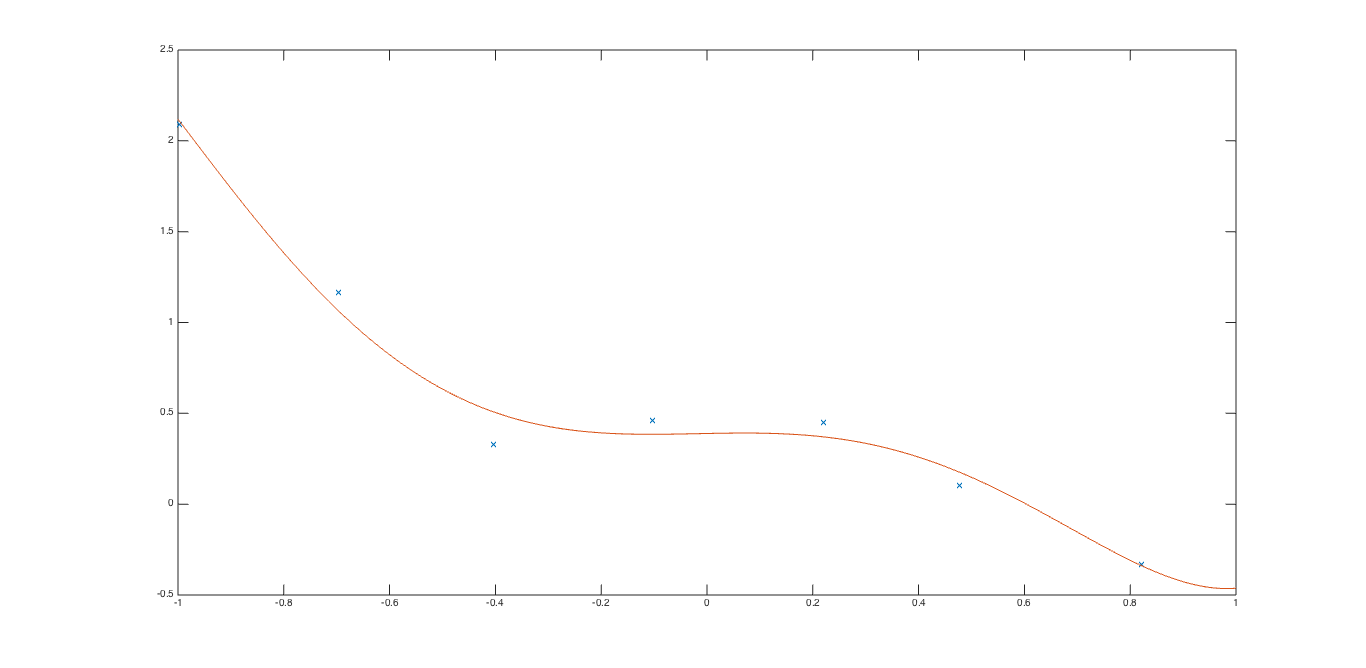
\includegraphics[width=1\textwidth]{PolynomialAlphaOnlyFunc}}
    \label{PolynomialAlphaOnlyFunc}
    \caption{Cost Function ($\alpha=1.461$)}
    \makebox[\textwidth]{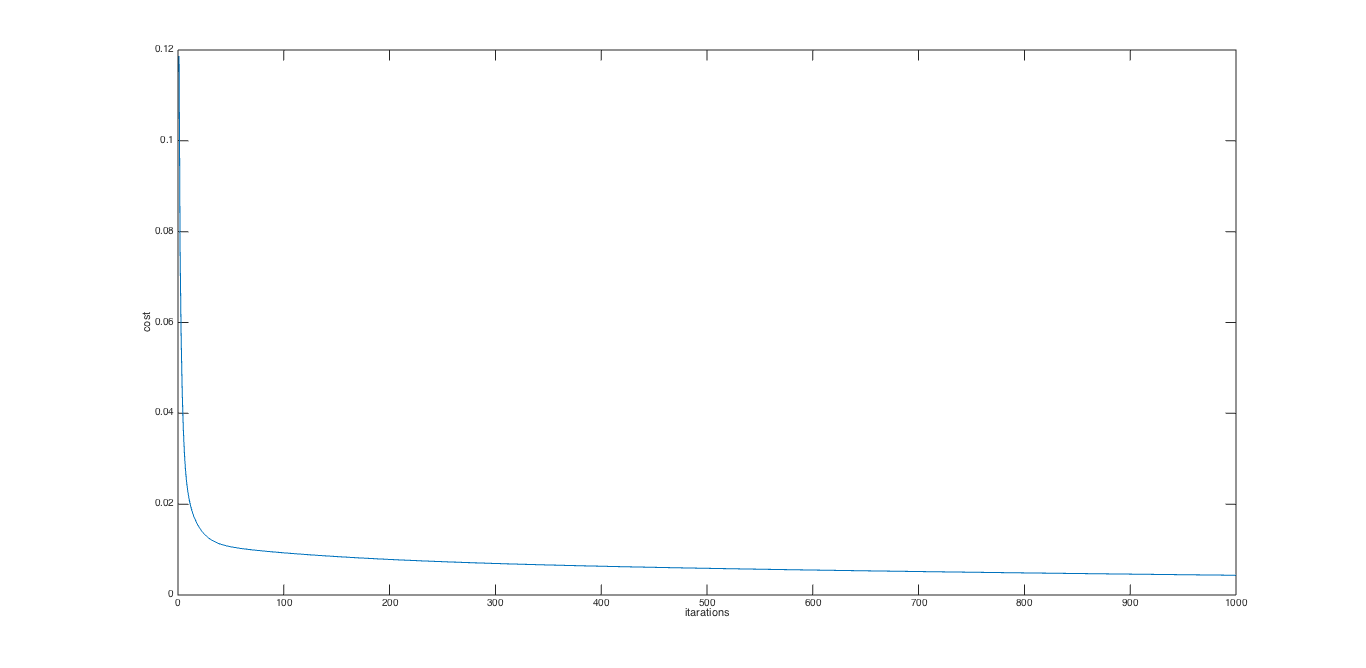
\includegraphics[width=1\textwidth]{PolynomialAlphaOnlyCost}}
    \label{PolynomialAlphaOnlyCost}
\end{figure}

\subsection{Experiment with different values of $\lambda$ and see how this affects the
    shape of the hypothesis.}
It appears that increasing value for $\lambda$ results in the flattening of the
hypothesis function. This is due to the penalisation of higher order terms in
the calculation of the hypothesis function. The results of $\alpha=1.2,
\lambda=3.0$ is shown in figure~\ref{PolynomialAlphaLambdaFunc}.

\begin{figure}
    \caption{Hypothesis Function ($\alpha=1.2, \lambda=3.0$)}
    \makebox[\textwidth]{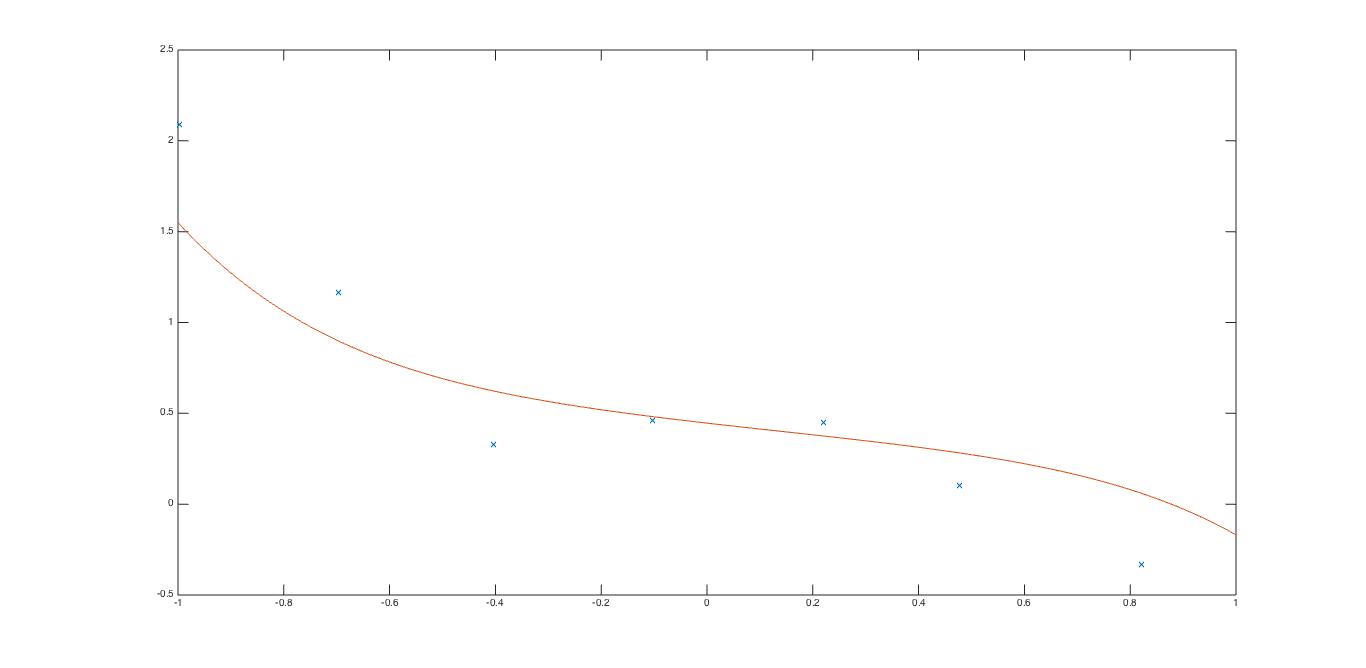
\includegraphics[width=1\textwidth]{PolynomialAlphaLambdaFunc}}
    \label{PolynomialAlphaLambdaFunc}
\end{figure}

% \printbibliography
\end{document}
